\chapter{Second Species of Counterpoint}

The second species of counterpoint consists of two notes by measure, two notes against one note. In other words, only half notes.
\begin{figure}[h]
    \centering
    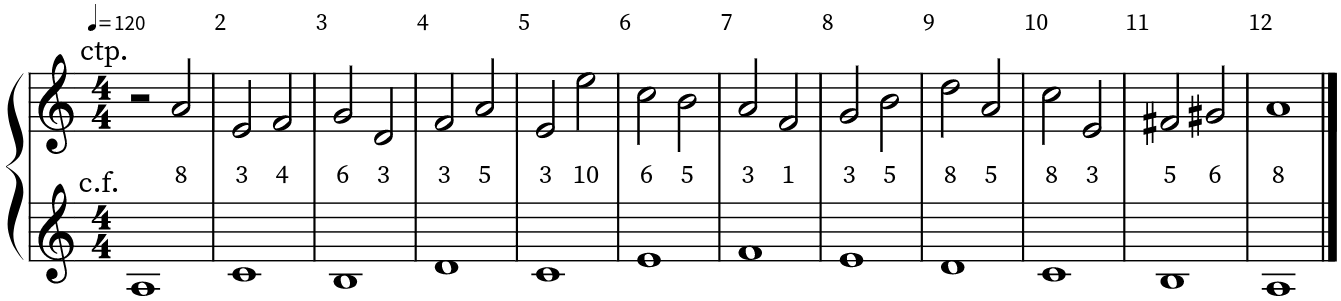
\includegraphics[height=\fhl]{Images/the_second_species.png}
    \caption{Example of a \species{2} ctp. \listen{Listen2SP} \listenyt{https://youtu.be/9yB4OGr4Cgk?t=70}}
\end{figure}

Since the second species is distinguished by a strong beat followed by a weak beat, the first species must be seen as a counterpoint composed of strong beats only. Therefore, all the rules of the first species that only apply per measure apply in thesis (e.g. rule \ref{rule:consthesis}). However, rule \ref{rule:mlesixth} applies generally with the exception \ref{rule:octaveleap}. Although the rules concerning the motions still hold, motions themselves are determined differently (see rule \ref{rule:motion2nd}).

To sum up, first species harmonic rules are applied in thesis, while first species melodic rules are applied for all notes, and first species motions rules are adapted to the species.

\section{Formalization in English}

\subsection{Harmonic Rules of the Second Species}

\begin{enumerate}[wide, label=\bfseries 2.H\arabic*]
    \item\label{rule:consthesis} \textit{Thesis\footnote{Thesis means the note on the down beat.} notes cannot be dissonant.} \textcite[p.64]{GaPFr}
    
    As explained above, this rule is consistent with the \ref{rule:allcons} one. Actually, it is written only to illustrate the associated logic because, in terms of constraints, the same are applied.

    \item\label{rule:arsisdim} \textit{Arsis\footnote{Arsis means the note on the upbeat.} harmonies cannot be dissonant except if there is a diminution\footnote{Diminution means an intermediate note that exists between two notes separated by a skip of a third.}.} \parencite[p.64]{GaPFr} 

    This might sound like a very restrictive rule but in reality, it is a common rule that applies itself in tonal music. In fact, any dissonance is surrounded by a consonance on each side.
    \begin{figure}[h]
        \centering
        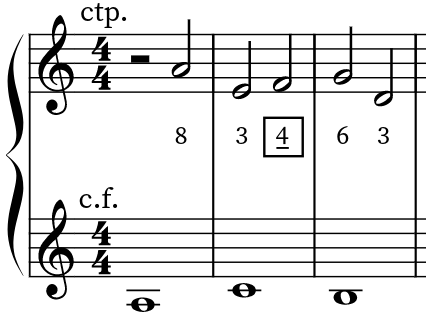
\includegraphics[height=\fh]{Images/diminution_arsis.png}
        \caption{Diminution in arsis, \species{2}.}
        \label{fig:diminutionarsis}
    \end{figure}

    Since rule \ref{rule:smallmelody} insinuates that the melodic intervals are small, it makes perfect sense to go from one thesis consonance to the next thesis consonance through an arsis dissonance.

    \item\label{rule:penult2nd} \textit{In addition to rules \ref{rule:low_penult} and \ref{rule:up_penult}, in the penultimate measure the harmonic interval of perfect fifth (unless exception \ref{rule:penultexception}) must be used for the thesis note.} \parencite[p.64-65]{GaPFr}

    The rules of the penultimate measure, although too strict for today's music (see rule \ref{rule:low_penult}), are still consistent with the other rules of the species. Since the penultimate note is a major sixth or a major third, the closest consonance in thesis is a fifth\footnote{With respect to the trend \ref{rule:smallmelody} that says that the melody is stepwise.} (see figure \ref{fig:penultmeasure2nd}).
    \begin{figure}[h]
        \centering
        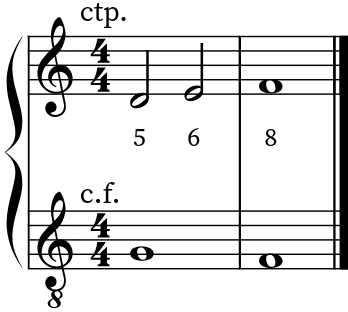
\includegraphics[height=\fh]{Images/penult_2nd.png}
        \caption{Basic penultimate measure, \species{2}.}
        \label{fig:penultmeasure2nd}
    \end{figure}

    \item\label{rule:penultexception} \textit{In the penultimate measure, if the harmonic interval of fifth in thesis is not available, then a sixth interval must be used.} \parencite[p.69]{GaPFr}

    When Fux makes exceptions, it can get tricky so it is highly recommended to understand rules \ref{rule:samekey} and \ref{rule:keytone} and the notion of modes. It should also be noted that, at the end of Fux's examples, the \cf tends to fall while the counterpoint tends to rise. It makes sense because the last motion must always be contrary\footnote{Or oblique in some cases. In Fux's examples, most of them tend to confirm this trend for the last two or even three notes of the counterpoint depending on the species. The examples given in this thesis are therefore strongly influenced by this idea which is omnipresent in the \citetitle{GaPFr}.}.

    Every musician knows that the seventh of the diatonic major scale does not have a perfect fifth in its key. That's why this rule exists. In figure \ref{fig:penultexsixth}, the mode of $E$ (i.e. the Phrygian mode) is used and the \cf plays an $F$ above. To have a perfect fifth, a $B\flat$ would have to be played, which is not available and is therefore replaced by an $A$ to form a sixth.

    \begin{figure}[h]
        \centering
        \begin{subfigure}{.5\textwidth}
            \centering
            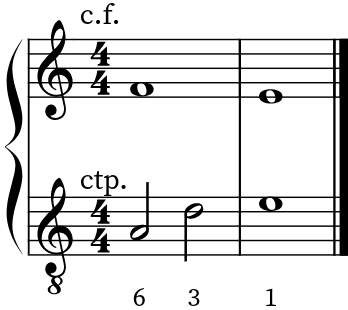
\includegraphics[height=\fh]{Images/penult_2nd_sixth.png}
            \caption{\nth{6} in thesis.}
            \label{fig:penultexsixth}
        \end{subfigure}%
        \begin{subfigure}{.5\textwidth}
            \centering
            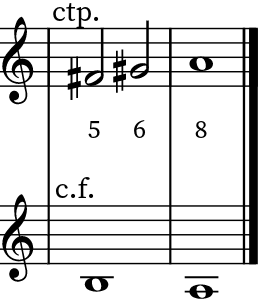
\includegraphics[height=\fh]{Images/penult_2nd_sharped.png}
            \caption{$\sharp$\nth{5} in thesis.}
            \label{fig:penultexfifth}
        \end{subfigure}
        \caption{Different penultimate measures, \species{2}.}
    \end{figure}

    Where it gets tricky is when Fux shows this example (figure \ref{fig:penultexfifth}) using the $A$ mode (i.e. the aeolian mode, the relative minor). Why does Fux allow himself to use $F\sharp$ which gives a perfect fifth to $B$? As always the key used is $C$ major (no $\sharp$ or $\flat$), but since the tonic is $A$ the scale used will be extended to notes of the $A$ major scale (i.e. $F\sharp$ and $G\sharp$)\footnote{For more experienced musicians, this penultimate measure is immediately reminiscent of the melodic minor scale \parencite{Minori}, which is common in classical music.}.

    One might ask: why not a sixth as in the first example (figure \ref{fig:penultexsixth})? There are two reasons for this choice. First, the implicit rule \ref{rule:chromafb} that says chromaticism is forbidden prevents a minor sixth because the melody would then be: $G \to G\sharp \to A$. Secondly, it could suggest that Fux prefers to go outside the diatonic scale to get a perfect fifth if the mode allows it rather than breaking the ground rule \ref{rule:penult2nd}. More details regarding the costs will be given in the next mathematical section.

\end{enumerate}

\subsection{Melodic Rules of the Second Species}
\begin{enumerate}[wide, label=\bfseries 2.M\arabic*]
    \item\label{rule:octaveleap} \textit{If the two voices are getting so close that there is no contrary motion possible without crossing each other, then the melodic interval of the counterpoint can be an octave leap\footnote{The octave leap is quite natural and easy to sing because it is the first harmonic of the sound \parencite{Octavewiki}.}.} \parencite[p.67-68]{GaPFr}

    \begin{quotation}
        "[\dots] if the parts have been led so close together that one does not know where to take them; and if there is no possibility of using contrary motion, this motion can be brought about by using the skip of [\dots] an octave [\dots]."
        \textcite[p.45]{GaPEng}
    \end{quotation}
    More explicitly, this case occurs when:
    \begin{itemize}
        \item the brut harmonic gap is a third or less;
        \item the \cf is both below (/above) and rising (/falling).
    \end{itemize}
    Why a third? Because there is no more closed consonance than the latter\footnote{Indeed, if the two voices are close, it is not possible to have a consonance other than unison (to be avoided) in this case.}.

    According to Fux's examples, this rule applies only to $thesis\to arsis$ melodic intervals. Octave leaps seem to be unconditional in the case of $arsis\to thesis$ intervals. Moreover, it goes hand in hand with rule \ref{rule:smallmelody} which says that melodic intervals should be small. Indeed, the octave skip allows to reset the pitch of the melody to go down (or up) again stepwisely (see figure \ref{fig:octaveleap}).
    \begin{figure}[h]
        \centering
        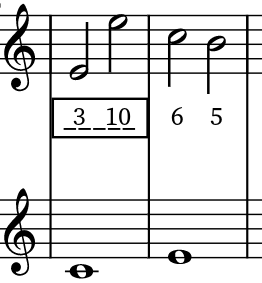
\includegraphics[height=\fh]{Images/octave_leap.png}
        \caption{Octave leap, \species{2}.}
        \label{fig:octaveleap}
    \end{figure}

    \item\label{rule:notsamecons} \textit{Two consecutive notes cannot be the same.*\footnote{"*" means that this rule is implicit.}}\\
    In Fux's examples, none of them have oblique motions. This makes sense with the criticisms made for rule \ref{rule:codmotions}. This rule applies to the third species.
\end{enumerate}

\subsection{Motion Rules of the Second Species}
\begin{enumerate}[wide, label=\bfseries 2.P\arabic*]
    \item\label{rule:motion2nd} \textit{If the melodic interval of the counterpoint between the thesis and the arsis is larger than a third, then the motion is perceived based on the arsis note.} \parencite[p.65-67]{GaPFr}

    Fux explains that the melodic interval between the note in thesis and the note in arsis determines which note will be kept in our mind. A third skip does not deviate enough from the thesis note to forget the latter. This implies that a perfect consonance to a perfect consonance cannot be saved by a third skip (see figure \ref{fig:thirdleap}) because the motion will be considered direct, which is not in accordance with rule \ref{rule:nopconsbydm}. However, this rule allows the following situation in figure \ref{fig:fourthleap}.

    \begin{figure}[h]
        \centering
        \begin{subfigure}{.5\textwidth}
        \centering
            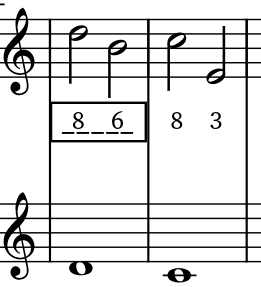
\includegraphics[height=\fh]{Images/bad_dm_2nd.png}
            \caption{Bad direct motion with a \nth{3} skip.}
            \label{fig:thirdleap}
        \end{subfigure}%
        \begin{subfigure}{.5\textwidth}
            \centering
            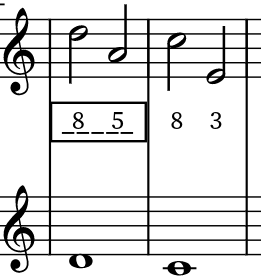
\includegraphics[height=\fh]{Images/good_dm_2nd.png}
            \caption{Good contrary motion with a \nth{4} leap.}
            \label{fig:fourthleap}
        \end{subfigure}
        \caption{Different motions based on different leaps, \species{2}.}
    \end{figure}

    \item\label{rule:battuta2} \textit{Rule \ref{rule:battuta} on the battuta octave is adapted such that it focuses on the motion from the note in arsis.*}

    Fux does not mention it in the second species. Instead of not applying the rule, it is adapted to prevent the same situation but considering only the note in arsis.
\end{enumerate}

\section{Formalization into Constraints}
\subsection{Harmonic Constraints of the Second Species}

\paragraph{\ref{rule:consthesis}} \textit{Thesis harmonies cannot be dissonant.}

As explained above, there is no constraint to add because it would be a duplicate of rule \ref{rule:allcons}.

\paragraph{\ref{rule:arsisdim}} \textit{Arsis harmonies cannot be dissonant except if there is a diminution.}

Let $IsDim$ be a list of booleans of size $m-1$ representing if an arsis note is a diminution. A diminution can be described as follows: the interval between the notes in thesis is a third and the two intervals that compose it are seconds (one or two semi-tones).

\begin{equation}
    \begin{gathered}
        \forj\\
        IsDim[j] = \begin{cases}
            \top & \text{if } M^2[0, j] \in \{3, 4\} \land M^1[0, j] \in \{1, 2\} \land M^1[2, j] \in \{1, 2\}\\
            \bot & \text{otherwise}
        \end{cases}
    \end{gathered}
\end{equation}

There is no need to use the brut melodic intervals to check if the melody always goes in the same direction\footnote{The note would be a mere ornament like a suspended or added note instead of a diminution.}. This is because the constraint of third ensures the conditions to be met: $M^2[0, j] = \left|M^1_{brut}[0, j] + M^1_{brut}[2, j]\right|$. Besides, the constraint $<= 2$ can be used to represent $\in \{1, 2\}$ because the melodic intervals are never zero as will be seen later.

\begin{lstlisting}[caption=Function that constrains $IsDim$ to reprensent diminutions., label=lst:dimin, basicstyle=\ttfamily\scriptsize]
; @m-intervals-ta: the melodic interval between each thesis and its following arsis
; @m-intervals: the melodic interval between each thesis and its following thesis
; @m-intervals-arsis: the melodic interval between each arsis and its following thesis
; @is-dim-arr: the array of BoolVar to fill
(defun create-is-dim-arr (m-intervals-ta m-intervals m-intervals-arsis is-dim-arr)
    (loop
    for mta in m-intervals-ta ; inter(thesis, arsis)
    for mtt in m-intervals ; inter(thesis, thesis + 1)
    for mat in m-intervals-arsis ; inter(arsis, thesis + 1)
    for b in is-dim-arr ; the BoolVar to constrain
    do (let (
        (btt3 (gil::add-bool-var *sp* 0 1)) ; s.f. mtt == 3
        (btt4 (gil::add-bool-var *sp* 0 1)) ; s.f. mtt == 4
        (bta-2nd (gil::add-bool-var *sp* 0 1)) ; s.f. mat <= 2
        (btt-3rd (gil::add-bool-var *sp* 0 1)) ; s.f. mtt == 3 or 4
        (bat-2nd (gil::add-bool-var *sp* 0 1)) ; s.f. mta <= 2
        (b-and (gil::add-bool-var *sp* 0 1)) ; temporary BoolVar
    )
        (gil::g-rel-reify *sp* mtt gil::IRT_EQ 3 btt3) ; btt3 = (mtt == 3)
        (gil::g-rel-reify *sp* mtt gil::IRT_EQ 4 btt4) ; btt4 = (mtt == 4)
        (gil::g-rel-reify *sp* mta gil::IRT_LQ 2 bta-2nd) ; bta-2nd = (mta <= 2)
        (gil::g-rel-reify *sp* mat gil::IRT_LQ 2 bat-2nd) ; bat-2nd = (mat <= 2)
        (gil::g-op *sp* btt3 gil::BOT_OR btt4 btt-3rd) ; btt-3rd = btt3 || btt4
        (gil::g-op *sp* bta-2nd gil::BOT_AND btt-3rd b-and) ; temporay operation
        (gil::g-op *sp* b-and gil::BOT_AND bat-2nd b) ; b = bta-2nd && btt-3rd && bat-2nd
)   ))
\end{lstlisting}

To represent an action that produces only in one situation, this action must imply that situation. So it can be established that a dissonance in arsis implies a diminution like this:

\begin{equation}
    \begin{gathered}
        \forj \quad
        \lnot IsCons[2, j] \implies IsDim[j]
    \end{gathered}
\end{equation}

\paragraph{\ref{rule:penult2nd}, \ref{rule:penultexception}} \textit{In the penultimate measure the harmonic interval of perfect fifth must be used for the thesis note if possible. Otherwise, a sixth interval should be used instead.}

If one wants to follow Fux's rules, it is important that the cost of leaving the diatonic scale is less than the cost of not having a fifth. For this, $cost_{penulthesis}$ is set to \dfts{last resort} which is greater than $cost_{OffKey}$ (\dfts{high cost}).

\begin{equation}
    \begin{gathered}
        H[0, m-2] \in \{7, 8, 9\}\\
        \therefore penulthesis_{cost} = \begin{cases}
            cost_{penulthesis} & \text{if } H[0, m-2] \neq 7\\
            0 & \text{otherwise}
        \end{cases}\\
        \text{moreover } \C = \C \cup penulthesis_{cost}
    \end{gathered}
\end{equation}

\subsection{Melodic Constraints of the Second Species}

\paragraph{\ref{rule:octaveleap}} \textit{If the two voices are getting so close that there is no contrary motion possible without crossing each other, then the melodic interval of the counterpoint can be an octave leap.}

\begin{equation}
    \begin{gathered}
        \forj, \forall M_{cf}[j] \neq 0\\
        M[0, j] = 12 \implies (H_{abs}[0, j] \leq 4) \land (IsCfB[j] \iff M_{cf}[j]>0)
    \end{gathered}
\end{equation}

Where $H_{abs}[0, j] \leq 4$ states that there is no smaller consonance and $IsCfB[j] \equiv M_{cf}[j]>0$ that the \cf is getting closer to the counterpoint. As a reminder, $M_{cf}$ is not absolute so $M_{cf}>0$ states that the \cf is necessarily rising.

\paragraph{\ref{rule:notsamecons}} \textit{Two consecutive notes cannot be the same.}

\begin{equation}
    \begin{gathered}
        \forp \quad
        Cp[\rho] \neq Cp[\rho+1]
    \end{gathered}
\end{equation}

\subsection{Motion Constraints of the Second Species}

\paragraph{\ref{rule:motion2nd}} \textit{If the melodic interval of the counterpoint between the thesis and the arsis is larger than a third, then the motion is perceived based on the arsis note.}

Let $P_{real}$ be a list of size $m-1$, with the same domain as a list of $P$, representing which motion is perceived between that coming from the thesis note and that coming from the arsis note. This implies that the costs of the motions and the first species constraints on the motions are deducted from $P_{real}$.

\begin{equation}
    \begin{gathered}
        \forj \quad
        P_{real}[j] = \begin{cases}
            P[2, j] & \text{if } M[0, j] > 4\\
            P[0, j] & \text{otherwise}
        \end{cases}
    \end{gathered}
\end{equation}

\begin{lstlisting}[caption=Function that constrains $P_{real}$ to represent the real motions., label=lst:realmotions, basicstyle=\ttfamily\scriptsize]
; @m-intervals-ta: melodic intervals between the thesis and the arsis note
; @motions: motions perceived from the thesis note
; @motions-arsis: motions perceived from the arsis note
; @real-motions: motions perceived by the human ear
(defun create-real-motions (m-intervals-ta motions motions-arsis real-motions)
    (loop
    for tai in m-intervals-ta
    for t-move in motions
    for a-move in motions-arsis
    for r-move in real-motions
    do (let (
        (b (gil::add-bool-var *sp* 0 1)) ; s.f. (tai > 4)
    )
        (gil::g-rel-reify *sp* tai gil::IRT_GR 4 b) ; b = (tai > 4)
        (gil::g-ite *sp* b a-move t-move r-move) ; r-move = (b ? a-move : t-move)
)   ))
\end{lstlisting}

\paragraph{\ref{rule:battuta2}} \textit{Rule \ref{rule:battuta} on the battuta octave is adapted such that it focuses on the motion from the note in arsis.}

This constraint already had an adapted mathematical notation in the chapter of the first species. Note that this constraint would indeed use $P[2]$ and not $P_{real}$.